\section{Arquitetura do sistema}


\subsection{Desenho do sistema}





\subsection{Nível 1}

\subsubsection{Diagrama Lógico}

\subsubsection{Diagrama de Implementação}

\subsubsection{Diagrama Físico} 

A figura \ref{fig:diagram-lvl1-physical} demonstra o diagrama de físico de nível 1. Utiliza-se o \textit{port} 80 pois este é por norma utilizado em chamadas \Acrshort{HTTP} por este um protocolo baseado em \ACRshort{TCP}

\begin{figure}[h!tbp]
    \centering
    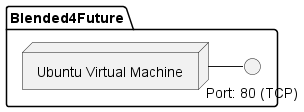
\includegraphics[width=0.5\linewidth]{capitulos/cap3-analisedoproblema/assets/arquiteturasistema/physical/physical_l1.png}
    \caption{Diagrama Físico de Nível 1}
    \label{fig:diagram-lvl1-physical}
\end{figure}





\subsection{Nível 2}

\subsubsection{Diagrama Lógico}

\subsubsection{Diagrama de Implementação}

\subsubsection{Diagrama Físico} 

A figura \ref{fig:diagram-lvl2-physical} demonstra o diagrama de físico de nível 2. Neste entende-se a função do servidor \gls{NGINX} como a de criação de duas rotas para \textit{Backend} e \textit{Frontend}, respetivamente \textit{'/api'} e \textit{'/'}.

\begin{figure}[h!tbp]
    \centering
    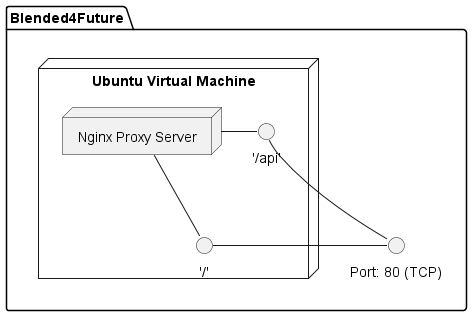
\includegraphics[width=0.6\linewidth]{capitulos/cap3-analisedoproblema/assets/arquiteturasistema/physical/physical_l2.png}
    \caption{Diagrama Físico de Nível 2}
    \label{fig:diagram-lvl2-physical}
\end{figure}


\subsection{Nível 3}

\subsubsection{Diagrama Lógico}

\subsubsection{Diagrama de Implementação}

\subsubsection{Diagrama Físico} 
A figura \ref{fig:diagram-lvl3-physical} demonstra o diagrama de físico de nível 3. Com este é possível verificar o mapeamento das duas rotas criadas pelo servidor \textit{proxy} \gls{NGINX} para os PORTS 3000 e 4000, escolhidos, pois são memoráveis. Foi feita ainda a escolha de encapsular as aplicações \textit{Backend} e \textit{Frontend} em imagens \gls{Docker} garantindo assim o seu funcionamento independentemente do \textit{hardware} escolhido.

\begin{figure}[h!tbp]
    \centering
    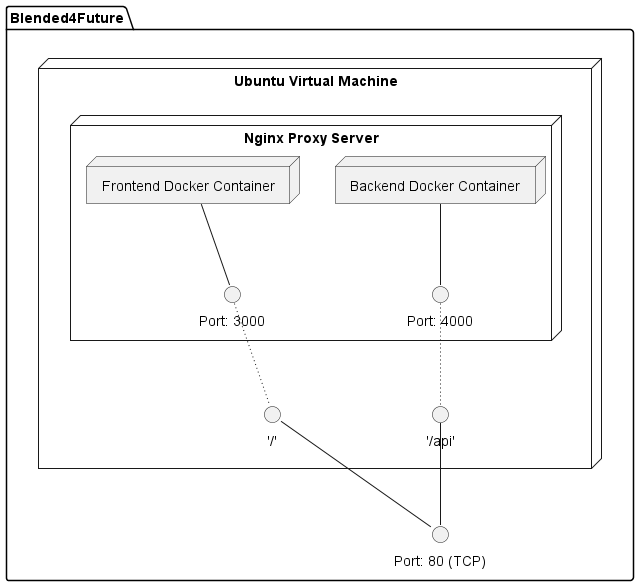
\includegraphics[width=0.7\linewidth]{capitulos/cap3-analisedoproblema/assets/arquiteturasistema/physical/physical_l3.png}
    \caption{Diagrama Físico de Nível 3}
    \label{fig:diagram-lvl3-physical}
\end{figure}





\subsection{Nível 4}

\subsubsection{Diagrama Lógico}

\subsubsection{Diagrama de Implementação}

\subsubsection{Diagrama Físico} 

A figura \ref{fig:diagram-lvl4-physical} demonstra o diagrama de físico de nível 4. Dento das respetivas imagens \gls{Docker} é possível as aplicações  \textit{Backend} e \textit{Frontend} encapsuladas. No contexto do \gls{Docker} é necessário fazer um mapeamento dos \textit{ports} utilizados do ambiente interno (Imagem) para o externo (Máquina Virtual), por isso é possível ver o mapeamento dos ports, respetivamente, internos e externos, 8080 e 4000, no \textit{Backend} e 3000 e 3000 no \textit{Frontend}.

Em nota, é possível incluir a base de dados na imagem graças à funcionalidade \textit{Volumes} do Docker e esta pode persistir diretamente no \textit{hardware} da máquina virtual.

\begin{figure}[h!tbp]
    \centering
    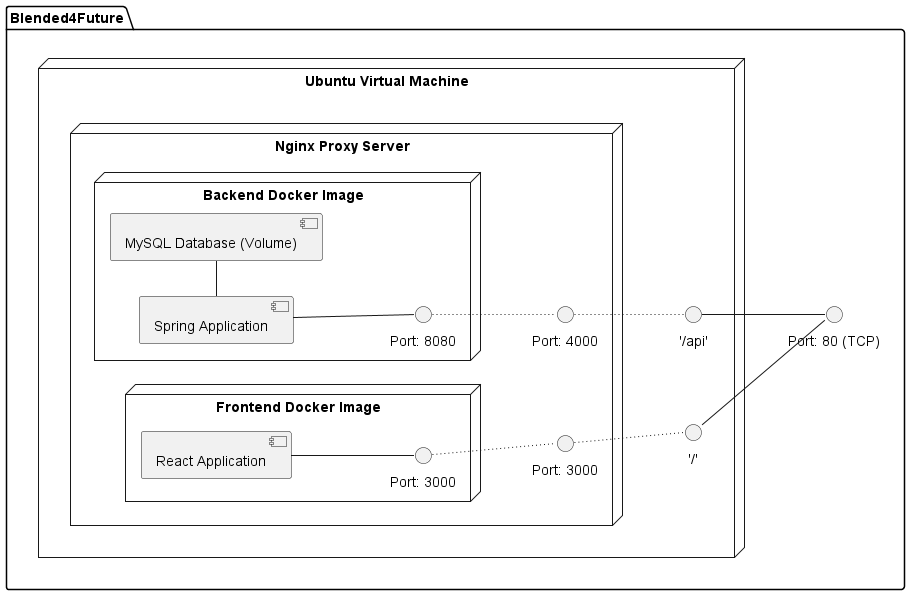
\includegraphics[width=\linewidth]{capitulos/cap3-analisedoproblema/assets/arquiteturasistema/physical/physical_l4.png}
    \caption{Diagrama Físico de Nível 4}
    \label{fig:diagram-lvl4-physical}
\end{figure}



\subsection{Padrões utilizados}
